The structure of the proposed control strategy is presented in \cref{fig:tikzControlStrat} and includes the aforementioned inner fast loop and outer slow loop:  

\begin{figure}[h!]
	\centering
	\resizebox{\columnwidth}{!}{
		\begin{tikzpicture}[auto, node distance=2.5cm,>=latex']
	% ========================== Nodes ============================
	% Nodes in upper vertical line
	\node [input, name=rinput] (rinput) {};
	\node [sum, right of=rinput] (sum1) {};
	\node [block, right of=sum1, node distance = 1.5cm] (LQR) {LQR};
	\node [sum, right of=LQR, node distance =
	1.5cm] (sum2) {};
	\node [block, right of=sum2, node distance = 1.5cm] (PID){PID};
	\node [block, right of=PID, align=center] (Fast){Fast\\Dynamics};
	\node [block, right of=Fast, node distance = 3cm, align=center] (Slow){Slow\\Dynamics};
	\node [output, right of=Slow] (output) {};
	
	% Nodes for inner feedback
	\node [tmp, right of=Fast, node distance = 1.5cm] (tmp0){};
	\node [tmp, below of=tmp0, node distance = 1.5cm] (tmp1){};
	\node [tmp, below of=sum2, node distance = 1.5cm] (tmp2){};
	
	% Nodes for outer feedback
	\node [tmp, right of=Slow, node distance = 1.5cm] (tmp10){};
	\node [tmp, below of=tmp10,node distance = 2.5cm] (tmp11){};
	\node [tmp, below of=sum1, node distance = 2.5cm] (tmp12){};
	
	% Nodes for Disturbance
	\node [tmp, above of=tmp0, node distance = 2.5cm] (tmp20){};
	\node [tmp, above of=tmp0, node distance = 2cm] (tmp21){};
	\node [tmp, above of=Fast, node distance = 2cm] (tmp22){};
	\node [tmp, above of=Slow, node distance = 2cm] (tmp23){};
	
	\draw[thick, dotted] ($(Fast.north west)+(-0.25, 0.25)$) rectangle  ($(Slow.south east)+(0.25, -0.25)$);
	\node[above of =tmp0, node distance =1.1cm](sys_txt) {System};
	
	% ========================== Lines ============================
	
	% Lines in upper vertical part of block diagram
	\draw [->] (rinput) -- node{$p_{ref}$} (sum1);
	\draw [->] (sum1) --node[name=z,anchor=north]{} (LQR);
	\draw [->] (LQR) -- node{$ q_{ref} $}(sum2);
	\draw [->] (sum2) -- (PID);
	\draw [->] (PID) -- node[pos=0.4]{$ \omega_{ref} $}(Fast);
	\draw [->] (Fast) -- node{$d_p$}(Slow);
	\draw [->] (Slow) -- node{$p_{\tau}$}(output);	
	
	% Lines for inner feedback
	\draw [-] (tmp0) -- (tmp1);
	\draw [-] (tmp1) -- (tmp2);
	\draw [->] (tmp2) -- node[pos=0.99]{$ - $}(sum2);
	
	
	% Lines for outer feedback
	\draw [-] (tmp10) -- (tmp11);
	\draw [-] (tmp11) -- (tmp12);
	\draw [->] (tmp12) -- node[pos=0.99]{$ - $}(sum1);
	
	
	% Lines for disturbance
	\draw [-] (tmp20)node[above, align=center]{Consumer \\ Disturbance} -- (tmp21);
	\draw [-] (tmp21) -- (tmp22);
	\draw [-] (tmp21) -- (tmp23);
	\draw [->] (tmp22) -- node[left, pos = 0.5]{$\Theta$}(Fast);
	\draw [->] (tmp23) -- node[pos = 0.5]{$ d_c $}(Slow);
	
	
\end{tikzpicture}
}
	\caption{Cascaded control strategy for fast and slow dynamics.}
	\label{fig:tikzControlStrat}
\end{figure}

\subsection{Outer Loop}\label{subsec:OuterLoop}

We will first address the outer VF-LQR controller. Its structure departs significantly from the classical LQR controller \cite{Skogestad2005}, as we use the velocity form proposed by \cite{Pannocchia2001}:

\begin{equation}\label{eq:LagrangeProblemDeviation}
	\begin{gathered}
	J = \sum_{k_0}^{\infty} \big(\zeta(k)^TQ\zeta(k) + \tilde{u}(k)^TR\tilde{u}(k)\big) \\
	\zeta = \begin{bmatrix}	x(k)-x(k-1) \\ y(k)-r(k) \end{bmatrix}, \quad \tilde{u}(k) = u(k)-u(k-1) 
	\end{gathered}
\end{equation} 

where the constraining dynamics are given by:

\begin{equation}\label{eq:VelocityMatrices}
	\begin{gathered}
		\zeta(k+1) = \tilde{A}\zeta(k) + \tilde{B}\tilde{u}(k) \\
		\tilde{A} = \begin{bmatrix} A & 0 \\ CA & I	\end{bmatrix}, \ 
		\tilde{B} = \begin{bmatrix} B \\ CB	\end{bmatrix}, \ \tilde{C} = \begin{bmatrix} 0 & I	\end{bmatrix}
	\end{gathered}
\end{equation}

and the optimal control policy becomes:

\begin{equation}\label{eq:OptimalVF-LQRPolicy}
\begin{gathered}
\tilde{u}^*(k)  = -\tilde{K}\tilde{x}^*(k) \\
\tilde{K} = (\tilde{B}^TP\tilde{B}-R)^{-1}(\tilde{B}^TP\tilde{A}) \\
u^*(k) = \sum_{i=1}^{k} \tilde{u}^*(i)
\end{gathered}
\end{equation}

where $P$ is the solution to the discrete algebraic Riccatti equation and the pairs $(A,B)$ and $(A,C)$ in \cref{eq:VelocityMatrices} are respectively controllable and observable, while $(Q,R)$ are positive semidefinite. This control policy clearly has tracking as $\zeta(k+1) = 0$ implies $y(k+1)-r(k+1) = 0$, and has integral action by virtue of its incremental form. However, it lacks disturbance rejection. Assuming that we are only concerned with optimal control of the disturbance-free subsystem, complete rejection of the state disturbance $\delta(k)$ can be achieved by augmenting \cref{eq:OptimalVF-LQRPolicy} \cite{Singh2017}:

\begin{equation}
	u(k) = \sum_{i=1}^{k} \tilde{u}^*(i) - B^\dagger \mathcal{B}\delta(i)
\end{equation}

where $B^\dagger$ is the Moore-Penrose pseudoinverse of $B$ and $\mathcal{B}$ is the disturbance input matrix. The value of this disturbance can be estimated by exploiting the knowledge that consumer demand is often approximately cosinusoidal \cite{Anele2017}, and building a disturbance estimator based on the model $\hat{d}_c = \beta + \alpha\cos(\omega t)$, which in the single-frequency case can be represented by the state-space model:

\begin{equation}\label{eq:TheisticDisturbanceEstimator}
	\begin{gathered}
		\dot{x} = A_\delta x =  \begin{bmatrix}0 & 0 & 0 \\ 0 & 0 & -\omega \\ 0 & \omega & 0	\end{bmatrix}x \\
		\hat{d}_c = C_\delta x = \begin{bmatrix} 1 & 1 & 0 \end{bmatrix} x
	\end{gathered}
\end{equation}

where $x = \begin{bmatrix}\beta & \alpha \cos(\omega t) & \alpha \sin(\omega t)\end{bmatrix}^T$. If this is discretised with Euler's method, the state equation becomes:

\begin{equation}\label{eq:TheisticDisturbanceEstimatorDiscrete}
	x(k+1) = \Big(I_{n\times n} + A_\delta t_s \Big) x(k) = \mathcal{A}_\delta x(k)
\end{equation}

and a discrete-time Kalman filter (KF) can then be constructed from $\{\mathcal{A}_\delta,C_\delta\}$ and appropriate noise models. \Cref{eq:TheisticDisturbanceEstimator} can be extended to the multi-frequency case by block-diagonal concatenation of several signal models, i.e. in the two-frequency case:

\begin{equation}\label{eq:DisturbanceVectorCase}
	\begin{gathered}
		\begin{bmatrix} \beta \\ \dot{x}_1 \\ \dot{x}_2 \end{bmatrix} = \begin{bmatrix} 0 & 0 & 0 \\ 0 & A_{\delta_1} & 0 \\ 0 & 0 & A_{\delta_2} \end{bmatrix} \begin{bmatrix}\beta \\ x_1 \\ x_2 \end{bmatrix},
		 \quad y = C_\delta \begin{bmatrix}\beta \\ x_1 \\ x_2 \end{bmatrix} \\
		 x_1, x_2 \in \mathbb{R}^{2\times1}, \quad {A}_{\delta_i} \in \mathbb{R}^{2\times2}, \quad
		 C_\delta \in \mathbb{R}^{1\times2n+1}
	\end{gathered}
\end{equation}

This signal model can then be combined with the expectation of mass conservation, which allows a proxy consumer flow measurement to be computed as $\hat{d}_c = d_p + d_\tau$.


\subsection{Inner Loop}\label{subsec:InnerLoop}

We now address the inner loop and its PI controllers. The model used for their design is the state-space model of the fast dynamics given in \cref{eq:LinearisedModelWithTank}, with a Padé approximation of a $4$-second output delay $T_{delay}$ included. This state-space system with output delay can be converted into the frequency-domain transfer matrix $G(s)$:

\begin{equation}\label{eq:TransferMatrix}
	G(s) = \begin{bmatrix} G_{11}(s) & G_{12}(s) \\ G_{21}(s) & G_{22}(s)\end{bmatrix}
\end{equation}

which can be shown to be approximately diagonal as per \cref{fig:BodeMagDelayPlot}:

\begin{figure}[h!]
 	\centering
 	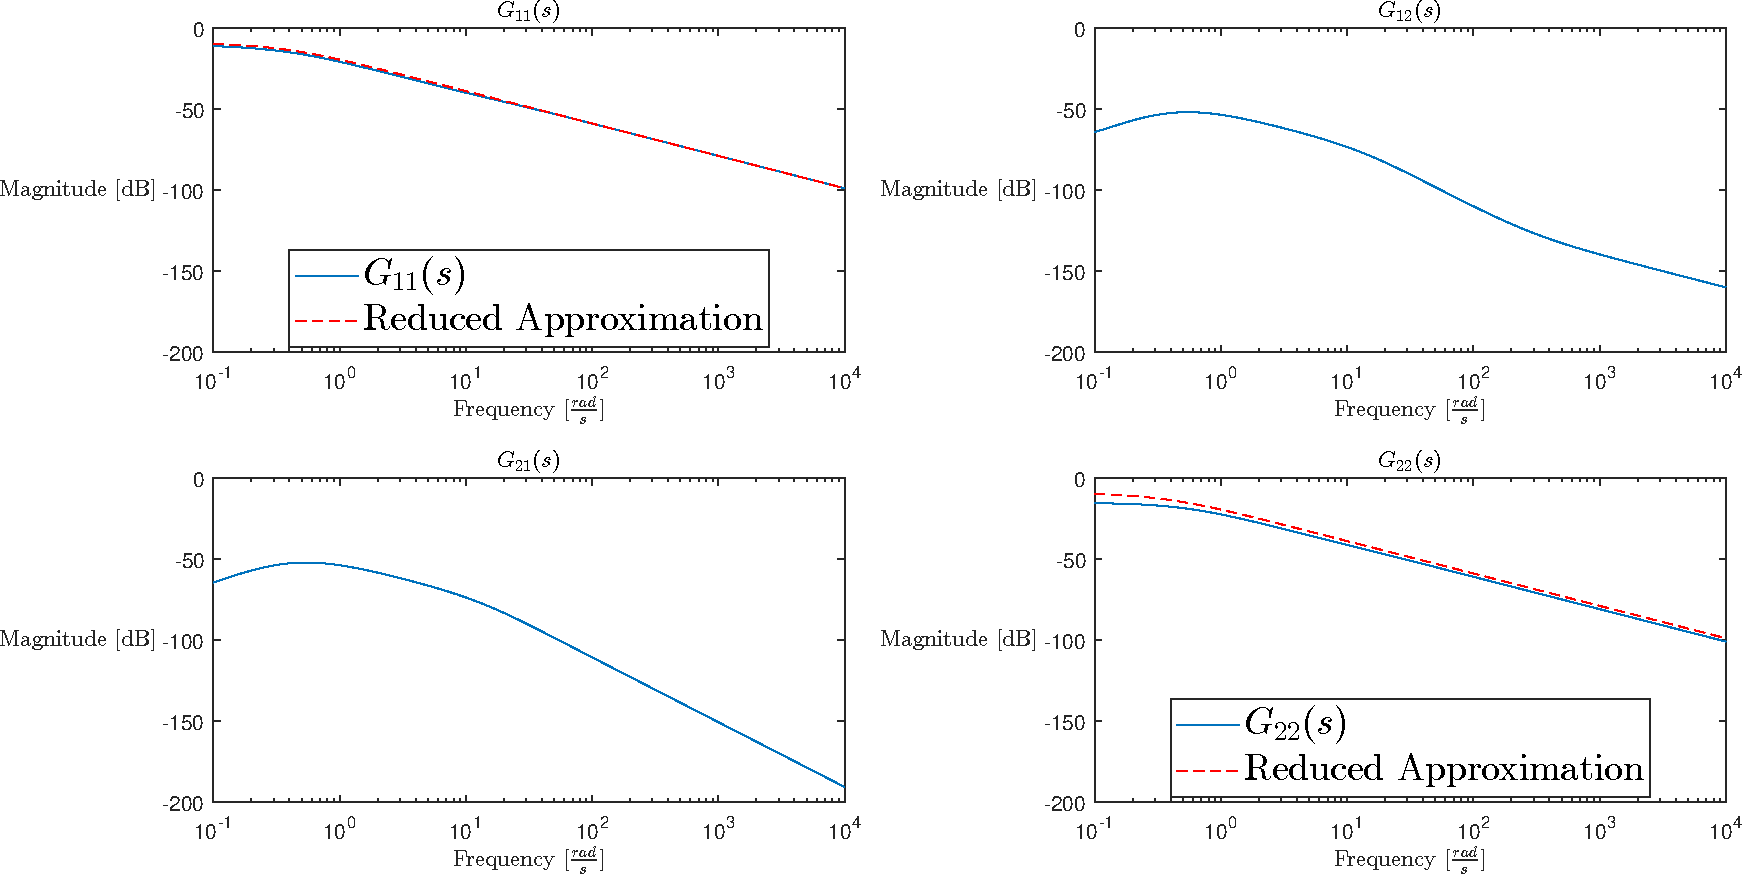
\includegraphics[width=\linewidth,height=4cm]{Graphics/PumpMagPlot.pdf}
 	\caption{Transfer matrix magnitude plots, output delay included.}
 	\label{fig:BodeMagDelayPlot}
\end{figure}

On account of this the PI controllers for pump speeds $\omega_1$ and $\omega_2$ can be designed as decentralised SISO controllers without decoupling. Their poles and zeros can, for design purposes be reduced to:

\begin{equation}\label{eq:PumpTFSimple}
	\begin{gathered}
		z_{11} = z_{22} = \begin{bmatrix}-0.19\end{bmatrix} \\
		p_{11} = p_{22} = \begin{bmatrix}-0.39 & -0.16 \end{bmatrix}
	\end{gathered}
\end{equation}

A PI controller is designed via the root-locus method with the goal of no overshoot to avoid ringing and accompanying pressure oscillations in the pipes. To accommodate the presence of an outer loop and allow this to operate at a reasonable sample rate, a bandwidth of $0.05 \frac{\si{rad}}{\si{s}}$ is chosen. Note that per \cite{Skogestad2005}, a stable controller cannot be designed with a closed-loop bandwidth higher than $\frac{1}{T_{delay}} = 0.25 \frac{\si{rad}}{\si{s}}$. The resulting controller is:

\begin{equation}\label{eq:PIDTransferFunction}
	C(s) = \frac{K_ps+K_i}{s} = \frac{1.8s+0.225}{s}
\end{equation}

\subsection{Outer Loop Stability Under Packet Loss}\label{subsec:PacketLossStability}

Because the outer and inner loops of the proposed control structure are likely to be located some physical distance from each other, and may be communicating over WiFi, stability analysis of the outer loop must take packet loss into account.

Anmon Sheth et al. \cite{Sheth2007} have shown that WiFi-based Long Distance Networks (WiLD) in urban environments suffer loss rates scaling exponentially with distance, from a worst-case loss rate of $7\%$ at $2\si{km}$, $15\%$ at $8\si{km}$, to $60\%$ at $20\si{km}$. Considering these losses as an upper bound $\alpha$ on possible loss, Hu and Yan \cite{Hu2007} give a sufficient condition for the stability of the outer loop in the mean-square sense if a Try-Once-Discard (TOD) protocol is assumed:

\begin{equation}\label{eq:HuStabCondition}
	\mathcal{S}\Big(\alpha A \otimes A + (1-\alpha)(A-BK) \otimes (A-BK) \Big) < 1
\end{equation}

where $\mathcal{S}$ is the spectral radius and $\otimes$ is the Kronecker product. Applying this theorem, we can show that the VF-LQR system is stable for the given values of packet loss, with spectral radii of $\{0.9238,0.9271,0.9453\}$. In fact, we can show that VF-LQR control of an arbitrarily sized tank is stable for \textit{any} value of packet loss in the zero limit of $\tilde{K}$. Assuming that the nominal, loss-free system is stable, applying Theorem 6 in \cite{Hu2007} gives the upper stability bound $\Xi$ as: 

\begin{equation}\label{eq:VMatrix}
	\begin{gathered}
		\Xi = \frac{1}{\lVert\sigma_+(V)\rVert_\infty} \\
		V = \begin{bmatrix} (S\otimes\hat{S}+\hat{S} \otimes S)(I - S\otimes S)^{-1} & \hat{S}\otimes\hat{S} \\ (I - S\otimes S)^{-1} & 0 \end{bmatrix} \\
		S = \left(\tilde{A}-\tilde{B}\tilde{K}\right) \otimes \left(\tilde{A}-\tilde{B}\tilde{K}\right), \quad \hat{S} = \tilde{A} \otimes \tilde{A} - S
	\end{gathered}
\end{equation}

Where $\sigma_+$ is the positive subset of the spectrum of $V$ and $\lVert \cdot \rVert_\infty$ is the infinity norm. Recalling due to \cref{eq:DiscreteTankPressureStateSpace} that $\tilde{A} \equiv \begin{bmatrix} 1 & 0 \\ 1 & 1 \end{bmatrix}$ for an arbitrary EWR, it can be shown that:

\begin{equation}\label{eq:AsymptoticPacketLossTolerance}
	\forall \alpha: \ \lim_{\tilde{K} \to 0} \mathcal{S}\Big(\alpha \tilde{A} \otimes \tilde{A} + (1-\alpha)(\tilde{A}-\tilde{B}\tilde{K}) \otimes (\tilde{A}-\tilde{B}\tilde{K}) \Big) = 1
\end{equation}

and thus that:

\begin{equation}\label{eq:AsymptoticXiBound}
	 \lim_{\tilde{K} \to 0} \Xi = 1
\end{equation}

which is an intuitive result for any system that describes an integrator at the origin.


